\section{Methods}
\label{sec:methods}

\subsection{Threat model}
We consider the following adversaries.
\begin{description}
	\item[Network-level adversary] An adversary that monitors at least
		one autonomous system, e.g., ISP, VPS provider, government.
	\item[Relay-level adversary] An adversary that runs at least one Tor relay.
	\item[DNS provider] An adversary that operates the DNS resolver used
		by exit relays, e.g., Google.
	\item[Active] To which extent to we consider active, content-modifying
		adversaries?  Attackers that see DNS can poison response and redirect
		victim to attacker-controlled domain.  That turns problem into trivial,
		classical end-to-end correlation.  Still, probably reason enough to tell
		exit relays that they should use DNSSEC.  Also, we might spot these
		attacks using exitmap.
\end{description}

We do not consider the case where Tor users misconfigure their client and leak
DNS requests unintentionally.

\subsection{Measuring AS exposure of DNS queries}
\label{sec:as-exposure}
How many more ASs do DNS queries traverse than subsequent web traffic?  If a
network adversary can see both types of traffic, she can ignore DNS because she
would do just fine with traditional TCP-based correlation attacks.  But if a
network adversary can only observe DNS traffic, she would have to invest in our
more complex attack to correlate streams.  We are interested in how many
adversaries are in this situation, i.e., how many ASs see DNS traffic, but no
web traffic.

We quantify the exposure of DNS compared to web traffic as follows.  We begin
with Alexa's Top 1,000, a list of the 1,000 most popular web sites as seen by
the Alexa search engine.  For each web site, we conduct two experiments.  First,
we run a TCP traceroute to the site, targeting port 80 to mimic web traffic.
Second, we determine the site's DNS delegation path using the dig command's
\texttt{+trace} feature.  The delegation path of a FQDN, say www.example.com, is
a list of authoritative DNS servers, e.g., the authoritative server for .com
pointing to the authoritative server of example.com, pointing to the
authoritative server responsible for www.example.com.  We run UDP traceroutes to
each server in the delegation path, targeting port 53 to mimic DNS queries.

For both experiments, we then map all IP addresses that we observed in the
traceroute to AS numbers, and generate a set of traversed ASs for DNS
traceroutes ($\mathcal{D}$), and a set of traversed ASs for web traceroutes
($\mathcal{W}$).  We are interested in the fraction of ASs that are \emph{only}
traversed for DNS traffic, but \emph{not} for web traffic.  To this end, we
define an exposure metric $\lambda$ that Equation~\ref{equ:exposure} shows.  The
metric approaches 1 as the number of ASs that are only traversed for DNS
increases.

\begin{equation}
\label{equ:exposure}
\lambda \in [0, 1] =
\frac{|\mathcal{D} \setminus \mathcal{W}|}
     {|\mathcal{D} \cup \mathcal{W}|}
\end{equation}

For example, if $\mathcal{D} = \{1,2,3\}$ and $\mathcal{W} = \{2,3,4\}$, then
$\lambda = \frac{|\{1\}|}{|\{1,2,3,4\}|} = \frac{1}{4} = 0.25$.  We determine
$\lambda$ for each site in the Alexa Top 1,000.  We ran these experiments on a
French VPS in AS 16276, owned by OVH SAS.  We chose this AS because as of April
2016, it is the most popular AS by exit bandwidth.  It sees $8.88\%$ of exit
traffic, closely followed by AS 3223 that sees $8.79\%$ of exit traffic.  The
result of the experiment is 1,000 $\lambda$ values.  We ran the same experiment
on a vantage point at our instutition, achieving similar results: While a
two-sample Kolmogorov-Smirnov test determined a statistically significant
difference between both distributions ($p < 0.01$), the medians (0.590 and
0.584) and standard deviations (0.149 and 0.118) are similar.

Figure~\ref{fig:exposure} shows the empirical CDF of all 1,000 $\lambda$ values
that we calculated for Alexa's Top 1,000 web sites.  In total, this experiment
traversed 350 unique ASs for DNS and 339 unique ASs for web.  The figure shows
that for half of Alexa's Top 1,000 domains, DNS-only ASs account for around 70\%
of all traversed ASs.  Note that this result is only relevant for exit relays
that handle their own DNS resolution.  If they use a third-party resolver, what
matters is the ASs that are traversed between the exit relay and the DNS
resolver.  Since we are not able to run traceroutes from an exit relay, it is
difficult to estimate this number.

% d1 <- read.csv("top-1k-ddptr-2016-04-19-ovh.csv")
% ecdf(d1$exposure)(0.5)
% 0.3050672

\begin{figure}[t]
	\centering
	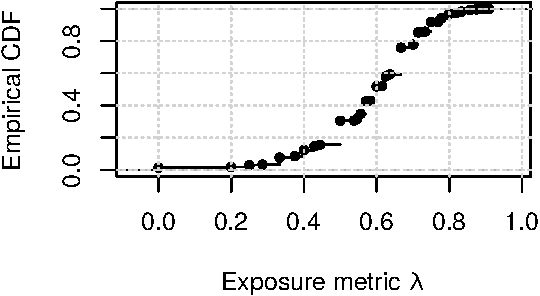
\includegraphics[width=0.75\linewidth]{figures/dns-exposure.pdf}
	\caption{Our AS exposure metric $\lambda$ for all web sites in the Alexa Top
	1,000.  For 50\% of all sites, DNS traffic traverses XXX times more ASs than
	web traffic.}
	\label{fig:exposure}
\end{figure}

\begin{figure}[t]
	\centering
	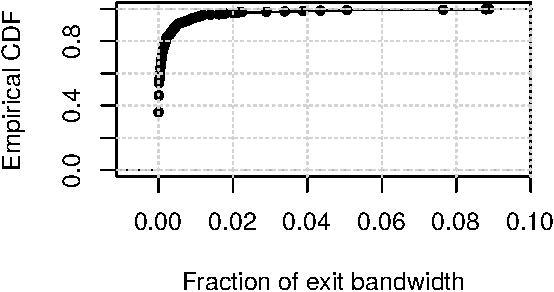
\includegraphics[width=0.75\linewidth]{figures/exitbw-per-as.pdf}
	\caption{The empirical CDF of the exit bandwidth for all ASs hosting exit
	relays as of April 2016.  Around 90\% of all ASs handle less than 1\% of
	exit bandwidth.  The top two ASs handle 8.88\% and 8.79\%, respectively.}
	\label{fig:exitbw-as}
\end{figure}

\begin{table}[t]
	\centering
	\begin{tabular}{l r r}
	\toprule
	\textbf{Type} & \textbf{Number of ASs} & \textbf{Percentage} \\
	\midrule
	DNS & 369 & 70.4 \\
	Web & 351 & 67.0 \\
	DNS $\setminus$ Web & 173 & 33.0 \\
	Web $\setminus$ DNS & 155 & 29.6 \\
	DNS $\cap$ Web & 196 & 37.4 \\
	DNS $\cup$ Web & 524 & 100.0 \\
	\bottomrule
	\end{tabular}
	\caption{The set relations between unique traversed ASs for DNS and unique
	traversed ASs for Web.}
	\label{tab:traversed-ass}
\end{table}

\subsection{Exposure at the Guard side}
\begin{itemize}
	\item Bad guards
	\item recognise dns requests by traffic analysis on the wire.  probably
		difficult because of optimistic data?  can we do more than just timing?
	\item can flow watermarking help?  see houmansadr's
		work~\cite{Houmansadr2011a}
\end{itemize}

\subsection{Mapping DNS resolvers}
As outlined in Section~\ref{sec:background}, Tor clients instruct exit relays to
establish a TCP connection to a hostname, and the exit relay simply responds
that the connection succeeded.  There is no way for Tor clients to learn what
DNS resolver handled name resolution.  Identifying these resolvers is a complex
task, and has not been covered in past work~\cite{Johnson2013a}.

For the first time, we answer this question by using exitmap~\cite{exitmap} and
our own DNS server.  Exitmap is a scanner for Tor exit relays.  It can execute
a task---e.g., the retrieval of a web page---over all one thousand exit relays,
allowing for seeing the Internet through the ``eyes'' of every single exit
relay.  Leveraging exitmap, we resolve unique, relay-specific domains over each
exit relay, to a DNS server under our control.  This experiment is visualized
in Figure~\ref{fig:dnsenum}.  To improve reliability, we configured exitmap to
use two-hop circuits instead of the standard three-hop circuits.  The first hop
was a guard relay under our control.  Over each exit relay, we resolve a unique
domain PREFIX.tor.nymity.ch whose authoritative DNS server we control.  The
prefix consists of the relay's unique 160-bit fingerprint concatenated to a
random 40-bit string whose purpose is to prevent caching, so exit relays indeed
resolve each query instead of responding with a cached element.  We control the
authoritative DNS server of nymity.ch, so we can observe the IP address and
packet content of every single query for nymity.ch.

\begin{figure}[t]
	\centering
	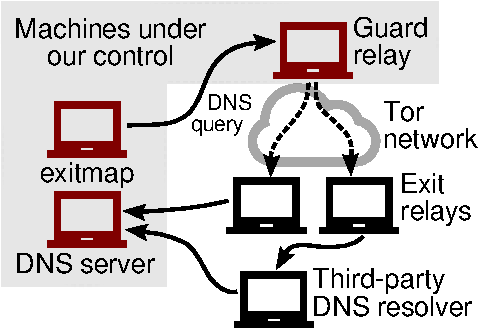
\includegraphics[width=0.8\linewidth]{figures/resolver-identification.pdf}
	\caption{Our method to identify the DNS resolvers of exit relays.  Over each
	exit relay, we resolve relay-specific domain names that are under our control.
	Inspecting our DNS server logs, we can then identify the IP address of all
	exit relay resolvers.}
	\label{fig:dnsenum}
\end{figure}

An exit relay can either run its own resolver (see the bottom relay in
Fig.~\ref{fig:dnsenum}), or use a third-party resolver such as the one provided
by its ISP (see the top relay in Fig.~\ref{fig:dnsenum}).  If an exit relay runs
its own resolver, we expect to receive a DNS request from the exit relay's IP
address, but if an exit relay uses a third-party resolver, we expect to receive
a request from an unrelated IP address.  Having encoded relay-specific
fingerprints in the query names, we are able to map queries to exit relays in
such cases.  We ran this experiment from September 2015 to \fixme{} 2016, six
times a day.  Finally, we encountered the following two difficulties.

\paragraph{DNS proxies}
Manual inspection of our data revealed that several exit relays used DNS
proxies, i.e., machines that passed on DNS requests to an actual resolver
instead of resolving it themselves.  Google's resolver 8.8.8.8 is a popular
example of a DNS proxy; the actual resolution is documented to be done by
several dozen machines in the background~\cite{google-proxies}.  It is
difficult to identify DNS proxies, so we ignored them in our data collection.
We believe that ignoring DNS proxies will not distort our results significantly
because we expect that proxies and resolvers are frequently located in the same
autonomous system.

\paragraph{Multiple DNS resolvers}
On Linux systems, DNS resolution is controlled by the file
\texttt{/etc/resolv.conf}.  It contains a list of up to three DNS resolvers
that are queried in order.  If the primary resolver does not respond within a
time limit, the system falls back to the second, and finally the third
resolver, if available.  Our data whos that several exit relays used different
resolvers in subsequent exitmap scans---one relay, for example, used both
Google's DNS resolver and one provided by its ISP.  For our visualization, we
only consider the first resolver we observed for an exit relay, which might not
be the primary resolver.  We believe that this method makes for the most
realistic estimate as the primary resolver handles the bulk of all DNS requests
of an exit relay.

\subsubsection{Visualizing results}
Figure~\ref{fig:exit-resolvers} illustrates the fraction of DNS requests that
all ASs that were ever in the top three could observe.  Google averages at
33\%, but at times it saw more than 40\% of all DNS requests exiting the Tor
network, a considerable number for a single organization.  Second to Google is
``Local,'' i.e., exit relays that run their own resolver, averaging at 12\%.
Next is OVH which used to be as popular as local resolvers, but slowly lost its
fraction over time.  Note that OVH resolvers are only meant for OVH customers,
and hence not public.  Between 0 and 5\% are seven more ASs, namely Level 3,
Visual Online, Init7, OpenDNS, Cyberdyne, NForce, and LeaseWeb.  Apart from the
illustrated top resolvers, the distribution has a long tail, presumably
consisting of many ISP resolvers.

\begin{figure*}[t]
	\centering
	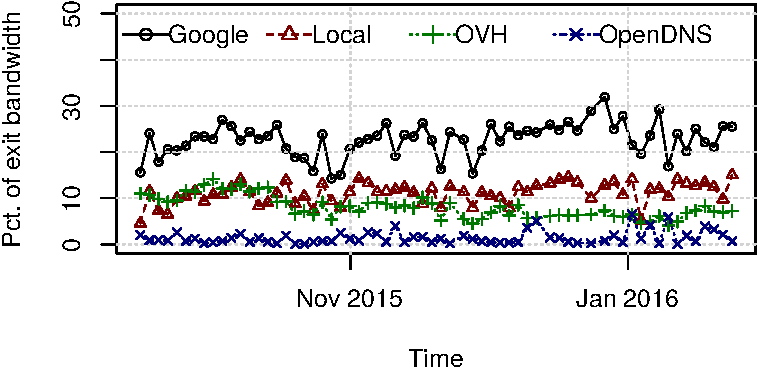
\includegraphics[width=\linewidth]{figures/exit-resolvers.pdf}
	\caption{The amount of the most popular DNS resolvers of exit relays over
	time, weighted by bandwidth.  Google's DNS server is by far the most popular
	resolver of exit relays, followed by a local resolver, OVH, and OpenDNS.
	The category ``Other'' consists of the ASs Level 3, Visual Online, Init7,
	OpenDNS, Cyberdyne, NForce, and LeaseWeb.}
	\label{fig:exit-resolvers}
\end{figure*}

\begin{table}[t]
	\centering
	\begin{tabular}{r l l}
	\toprule
	\textbf{Percentage} & \textbf{Organization} & \textbf{Country} \\
	\midrule
21.6 & Google & US \\ % -> 21.56 bw pct.
13.1 & Local resolver & --- \\ % -> 14.14 bw pct.
6.5 & OpenDNS & US \\ % -> 6.46 bw pct.
6.5 & OVH & FR \\ % -> 6.46 bw pct.
2.7 & S.A.S. & FR \\ % -> 2.65 bw pct.
2.5 & NFOrce Entertainment & NL \\ % -> 2.47 bw pct.
2.1 & UK2 & GB \\ % -> 2.07 bw pct.
2.0 & Iomart & GB \\ %  -> 1.96 bw pct.
1.9 & CYBERDYNE & LR \\ % -> 1.90 bw pct.
1.7 & DFRI & SE \\ % -> 1.74 bw pct.
% 1.7 & Level 3 Communications & US \\ % -> 1.72 bw pct.

% 	306 & 33.4\% & Google & US \\
% 	62 & 6.8\% & OVH SAS & FR \\
% 	26 & 2.8\% & OpenDNS & US \\
% 	23 & 2.5\% & Hetzner Online & DE \\
% 	18 & 2.0\% & S.A.S. & FR \\
% 	17 & 1.9\% & Hurricane Electric & US \\
% 	14 & 1.5\% & LeaseWeb Netherlands & NL \\
% 	12 & 1.3\% & Level 3 Communications & US \\
% 	8 & 0.9\% & Iomart & GB \\
% 	7 & 0.8\% & PlusServer & DE \\
% 	\hline
% 	71 & 7.7\% & Local resolver & \\
	\bottomrule
	\end{tabular}
	\caption{The top ten resolvers used by all exit relays by capacity on Jan 1,
	2016.  More than 20\% of all exit bandwidth at the time used Google's DNS
	server.  13.1\% of exit bandwidth is resolved by local DNS resolvers.}
	\label{tab:dns-resolvers}
\end{table}


\subsection{Mapping resolver configuration}
In addition to identifying an exit relay's DNS resolver, our technique can
ascertain parts of its configuration.  Resolvers with poor or broken
configuration pose a security risk to Tor users as attackers could poison or
enumerate their cache, allowing them to redirect users or profile them.
Therefore, it is important to identify broken resolvers because they jeopardize
the anonymity of Tor users.

\paragraph{Random source ports}
To impede cache poisoning attacks, DNS resolvers should use random source ports
instead of always using UDP port 53.  Our data allows for verifying if a given
resolver randomizes its source ports.  We classify a resolver as ``uses
randomization'' if the source port does not equal 53.  Note that this method
causes a small number of false positives because a randomizing resolver could
use port 53 simply by chance.  However, the probability of that happening is
only $\frac{1}{65535}$.

We found 135 DNS resolvers that did not use random source ports.  These
resolvers were located in the networks of Vodafone, Germany (95\%), MTNL, India
(4\%), and Cogent, U.S. (1\%).

\paragraph{0x20 encoding}
Resolvers can further reduce the chance of cache poisoning by employing 0x20
encoding, i.e., randomizing the capitalization of domain names.  For example, to
resolve foo.com, a resolver would send a request for fOo.CoM.  If the DNS
response does not reflect the randomly chosen capitalization, the resolver
considers unauthentic.  We classify a resolver as ``uses 0x20'' if it has at
least one lowercase and one uppercase character.  Again, there is a chance of
false positives, which depends on the domain name length.  A 0x20-encoded domain
name of $n$ characters (excluding periods) can be all-uppercase or all-lowercase
with probability $2 \cdot 0.5^n$.

We found 427 DNS resolvers that did not use 0x20 encoding for at least one
query.  The top five resolvers were located in the networks of Google, U.S.
(38\%), AT\&T, U.S. (22\%), Deutsche Telekom, Germany (7\%), Yandex, Russia
(7\%), OpenDNS, U.S. (4\%).

\paragraph{DNSSEC validation}
We can verify if a resolver is validating DNSSEC-signed records by resolving a
domain whose signature is deliberately malformed.  Such a service is provided by
dnssec-failed.org.  A validating resolver would not return an A record while a
non-validating resolver would.  Therefore, we resolve dnssec-failed.org over all
exit relays and check if we get an A record in response.

\subsection{Internet map}
\begin{itemize}
	\item Where do we get our AS and IXP graph from?
	\item Johnson et al.~\cite[\S 5.2]{Johnson2013a} used RouteViews and the CAIDA IPv4
		Routed /24 AS Links Dataset, resulting in 44,605 ASs connected by
		305,381 links.
\end{itemize}

\subsection{Traceroute dataset}
\label{sec:traceroute-dataset}
\begin{itemize}
	\item Find machines that are topologically close to DNS resolvers
		used by exit relays.
	\begin{itemize}
		\item RIPE Atlas probes.
		\item Virtual private systems.
		\item PlanetLab nodes.
		\item Ask exit operators to run traceroutes for us.
	\end{itemize}
	\item Run traceroutes to DNS servers to determine path coverage.
	\item Determine ``AS inflation factor.''
\end{itemize}

In this analysis we assume that an AS that can see traffic entering the Tor network and 
DNS traffic at the other end can use this information in order to deanonymize the 
entering traffic. Here we seek to measure the chances an AS will be in the ``correct'' 
position to carry out such an attack.

A Tor exit can carry out DNS name resolution in two different ways: it can either do it
itself by running a name server locally, or it can rely on a 3rd-party name server, 
such as its ISP's name server or a public DNS name server like Google's 8.8.8.8.

Let us examine these two different scenarios: local resolution vs. 3rd-party 
resolution. With local resolution, a good position for an AS is to be on the path between 
a Tor client and a Tor guard and on the path between a Tor exit and any of the name 
servers the exit has to communicate with in order to resolve the name. These name servers 
can include the root name server, the TLD servers, and the other ones**fix this. The ASes 
along the way from the exit relay to the name servers will be able to see the names that 
are being queried.

For 3rd party resolution, a good position for an AS is to be on the path between 
a Tor client and a Tor guard and on the path between the exit relay and that 3rd party 
name server. Beyond that, the queries will look like they're coming from the IP address 
of the name server and not the IP address of the exit relay, which is what we're interested 
in. 

In this analysis, we completely ignore caching of any type. TorPS is based on Tor version X. 
For each sample, it uses one guard which will expire after 270 days. We have TorPS simulate
the behavior of a Tor client for the month of March 2016.


\subsection{DNS packet sizes at entry guard}
\begin{itemize}
	\item Send many DNS requests over entry guard.
	\item Capture them on the wire and look at them.
	\item What's the best way to filter out the noise?
\end{itemize}

\subsection{Practical attacks}
We leverage the following building blocks:
\begin{itemize}
	\item Traffic analysis done on an entry guard.  Can DNS requests be isolated
		reliably?
	\item Access to DNS root, .com, and .net.
	\item Ability to use DNS resolver's cache as an oracle.
	\item Ability to enumerate what resolver's an exit relay uses.
	\item Resolvers using EDNS.
	\item Users in country X are likely to resolve domains of country X.
\end{itemize}
